\documentclass[a4paper,12pt]{article}
%%%%%%%%%%%%%%%%%%%%%%%%%%%%%%%%%%%%%%%%%%%%%%%%%%%%%%%%%%%%%%%%%%%%%%%%%%%%%%%%%%%%%%%%%%%%%%%%%%%%%%%%%%%%%%%%%%%%%%%%%%%%%%%%%%%%%%%%%%%%%%%%%%%%%%%%%%%%%%%%%%%%%%%%%%%%%%%%%%%%%%%%%%%%%%%%%%%%%%%%%%%%%%%%%%%%%%%%%%%%%%%%%%%%%%%%%%%%%%%%%%%%%%%%%%%%
\usepackage{eurosym}
\usepackage{vmargin}
\usepackage{amsmath}
\usepackage{graphics}
\usepackage{epsfig}
\usepackage{framed}
\usepackage{subfigure}
\usepackage{fancyhdr}

\setcounter{MaxMatrixCols}{10}
%TCIDATA{OutputFilter=LATEX.DLL}
%TCIDATA{Version=5.00.0.2570}
%TCIDATA{<META NAME="SaveForMode"CONTENT="1">}
%TCIDATA{LastRevised=Wednesday, February 23, 201113:24:34}
%TCIDATA{<META NAME="GraphicsSave" CONTENT="32">}
%TCIDATA{Language=American English}

\pagestyle{fancy}
\setmarginsrb{20mm}{0mm}{20mm}{25mm}{12mm}{11mm}{0mm}{11mm}
\lhead{MA4128} \rhead{Kevin O'Brien} \chead{Week 8 Part B} %\input{tcilatex}

%http://www.electronics.dit.ie/staff/ysemenova/Opto2/CO_IntroLab.pdf
\begin{document}

\tableofcontents
\newpage

\section{Output of Linear Regression Analysis}
Linear regression is used when you want to predict the value of a variable based on the value of another variable. The variable we want to predict is called the dependent variable (or sometimes, the outcome variable). The variable we are using to predict the other variable's value is called the independent variable (or sometimes, the predictor variable).
\[ \hat{y} = b_o + b_1 x \]
\begin{itemize}
\item $b_o$ is the intercept estimate
\item $b_1$ is the slope estimate
\item $\hat{y}$ is the \textbf{\textit{fitted}} y-value, given a specified value of the indepenent variable $x$.
\item The fitted value and the observed value of y often differ. This difference is known as the \textbf{\textit{residual}}
\end{itemize}

For example, you could use linear regression to understand whether exam performance can be predicted based on revision time; whether cigarette consumptions can be predicted based on smoking duration; and so forth. If you have two or more independent variables, rather than just one, you need to use \textbf{\textit{multiple regression}}.

SPSS will generate quite a few tables of output for a linear regression procedure. Only the three main tables required to understand your results from the linear regression procedure, assuming that no assumptions have been violated.

This includes relevant scatterplots, histogram (with superimposed normal curve) and Normal P-P Plot, and case-wise diagnostics and Durbin-Watson statistic tables. Below, we focus on the results for the linear regression analysis only.

\begin{figure}[h!]
\begin{centering}
  % Requires \usepackage{graphicx}
  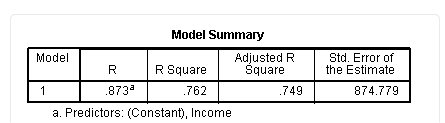
\includegraphics[width=10cm]{Regre4.jpg}\\
  \caption{Model Summary table}
\end{centering}
\end{figure}

The first table of interest is the \textbf{\textit{Model Summary}} table. This table provides the R and $R^2$ value. The R value is 0.873, which represents the simple correlation. It indicates a high degree of correlation. The $R^2$ value indicates how much of the dependent variable, \textbf{\textit{price}} (Not evident on output), can be explained by the independent variable,\textbf{\textit{income}}. In this case, 76.2\% can be explained, which is very large.


The next table is the ANOVA table. This table indicates that the regression model predicts the outcome variable significantly well. How do we know this? Look at the \textbf{\textit{Regression}} row and go to the \textbf{Sig.} column. This indicates the statistical significance of the regression model that was applied. Here,the p-value is  $p < 0.0005$, which is less than 0.05, and indicates that, overall, the model applied can statistically significantly predict the outcome variable.

\begin{figure}[h!]
\begin{centering}
  % Requires \usepackage{graphicx}
  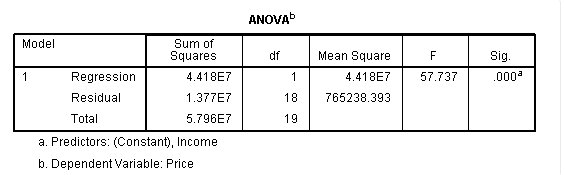
\includegraphics[width=10cm]{Regre5.jpg}\\
  \caption{ANOVA Table}
\end{centering}
\end{figure}

The next table again, \textbf{\textit{Coefficients}}, provides us with information on each predictor variable. This gives us the information we need to predict price from income. We can see that both the constant and income contribute significantly to the model (by looking at the Sig. column). By looking at the B column under the Unstandardized Coefficients column, we can present the regression equation as:

\textit{\textbf{ $\hat{Price}$ = 8287 + 0.564(Income)}}

\begin{figure}[h!]
\begin{centering}
  % Requires \usepackage{graphicx}
  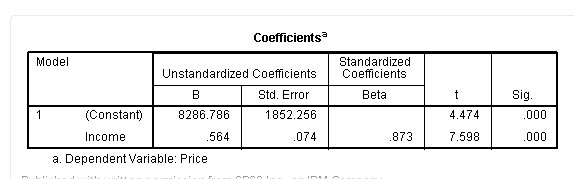
\includegraphics[width=10cm]{Regre6.jpg}\\
  \caption{Coefficients Table}
\end{centering}
\end{figure}


\newpage
\section{Multiple Linear Regression}
\subsection{What is Multiple Linear Regression}

Multiple regression is a statistical technique that allows us to predict a numeric value on the response variable on the basis of the observed values on several other independent variables.


\[\hat{y} = b_0 + b_1x_1 + b_2x_2 + \ldots \]

\begin{itemize}
\item $\hat{y}$ is the \textbf{\textit{fitted value}} for the dependent variable \textbf{$Y$}, given a linear combination of values for the independent valriables.

\item $x_i$ is the value for independent variable \textbf{$X_i$}. (For Example, $x_1$ is the value for independent variable \textbf{$X_1$}.)
\item $b_o$ is the constant regression estimate ( commonly known as the \textbf{Intercept Estimate} in the case of simple linear regression).
\item $b_i$ is the regression estimate for Independent Variable \textbf{$X_1$} ( commonly known as the \textbf{Slope Estimate} in the case of simple linear regression).
\end{itemize}

\subsubsection{Simple Example}
Suppose we were interested in predicting how much an individual enjoys their job. Independent Variables such as salary, extent of academic qualifications, age, sex, number of years in full-time employment and socioeconomic status might all contribute towards \textbf{\textit{job satisfaction}}.

If we collected data on all of these variables, perhaps by surveying a few hundred members of the public, we would be able to see how many and which of these variables gave rise to the most accurate prediction of job satisfaction. We might find that job satisfaction is most accurately predicted by type of occupation, salary and years in full-time employment, with the other variables not helping us to predict job satisfaction.


